\subsection{Li-Ion-Batterie}\label{sec:energiespeicher}

Die gesamte Energiespeicherung wird mit einem Lithium-Ionen-Akkumulator des Typs Emmerich LI14500 realisiert. Dieser weist eine Kapazität von $800mAh$ bei einer Nominalspannung von $3.7V$ auf und verfügt über interne Schutzeinrichtungen. Um eine Abschätzung über die Betriebszeit des Dōjōs zu erhalten, sind Faktoren wie maximaler Verbrauch, Nominalspannung und Kapazität notwendig. Die maximale Leistung des Dōjōs lässt sich durch die Leistung des Verstärkers/ Knochenschallgebers ($P_{Kn}$) und die des Mikrocontrollers ($P_{MC}$) beschreiben. Alle anderen Komponenten können aufgrund des geringen Betriebsstrom mit einem Sicherheitsfaktor ($P_{zus}$) von $0.1W$ dazu gerechnet werden. Die Leistung des Verstärkers weist eine maximale RMS-Leistung von $471.9mW$ auf. Gerechnet wird mit $80\%$ des RMS Wertes, da der Knochenschallgeber nicht permanent beansprucht wird. Die Leistungsaufnahme des Mikrocontrollers beträgt $27.36mW$ und wurde durch Messungen ermittelt. Die Gesamtleistung wird wie folgt berechnet:

\begin{equation}
\centering
P_{max}=\left(0.8\cdot P_{Kn}\right)+P_{MC}+P_{zus}=(0.8\cdot 0.472W)+(0.02736W)+0.1W=0.506W
\label{eq:MaxLeistung}
\end{equation}

Die Gesamtleistung beträgt somit rund $0.506 W$. Nun kann basierend auf der Gesamtleistung die Betriebszeit $t_{max}$ berechnet werden:

\begin{equation}
\centering
t_{max}=\frac{W\cdot U}{P_{tot}}=\frac{800mAh \cdot 3.7V}{506mW}=5.85h\approx 5h \thickspace 51min
\label{eq:Betriebszeit}
\end{equation}

Es ist somit ersichtlich, dass bei permanentem Einsatz eine maximale Betriebszeit von knapp 6 Stunden erzielt werden kann. Allerdings kann ein lückenloser Betrieb durch einen geschickten Ladeprozess erzielt werden.

\subsubsection*{Schutzeinrichtungen}\label{sec:schutzeinrichtung}
Um den verwendeten Akkumulator zu schützen, sind diverse Schutzeinrichtung notwendig. Zum einen muss der Ladevorgang überwacht werden, so dass der maximale Ladestrom wie auch die Ladespannung nicht überschritten werden. Für die Laderegelung wurde ein Lade-IC von Microchip des Typs MCP73831 verwendet. Dieser übernimmt die gesamte Spannungs- und Stromregelung beim Ladeprozess und kann parallel zum Ladevorgang eine LED zur Ladesignalisation ansteuern. Der Ladezyklus ist in der Abbildung  \ref{fig:Ladekurve Li-Ion Akku} ersichtlich. Hierbei wurde der Akku im Schnelllademodus mit einem maximalen Strom von $400mA$ geladen. Dieser Strom ergibt sich aus dem Datenblatt der Batterie \cite{LIBattery}, wobei sowohl der Entladestrom, als auch der Ladestrom 0.5 $\cdot$C pro Stunde beträgt. C entspricht der Batteriekapazität. Somit lässt sich der Strom folgendermassen berechnen:

\begin{equation}
\centering
I_{charge}={0.5 \dfrac{1}{h} \cdot 800mAh}= 400mA
\label{eq:Ladestrom}
\end{equation}

Betrachtet man die Abbildung \ref{fig:Ladekurve Li-Ion Akku}, so wird ersichtlich, dass die Spannung rund $2.5h$ geregelt wird bis 4.2V Grenze erreicht wird. Sobald der Spannungswert $4.2V$ erreicht hat, beginnt der Lade-IC mit der Stromregelung. Für diesen Prozess wurden beim Versuch noch einmal rund 30 Minuten benötigt, wodurch die letzten rund $20\%$ der Batteriekapazität geladen werden konnten.

\begin{figure}[H]
	\begin{center}
		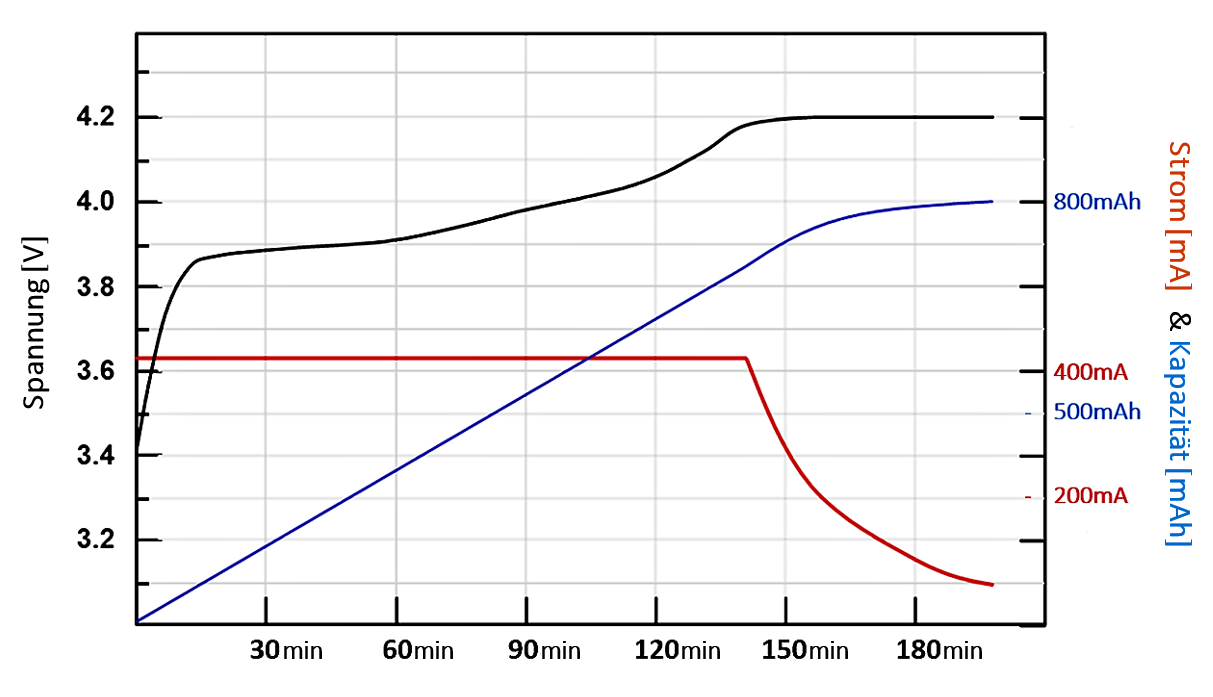
\includegraphics[width=120mm]{data/LadekurveLiIon.png}
		\caption[Ladekurve Li-Ion Akku]{Ladekurve Li-Ion Akku} %picture caption
		\label{fig:Ladekurve Li-Ion Akku}
	\end{center}
\end{figure}


Für einen weiteren Schutz, hat die Emmerich LI14500 eine integrierte Schutzbeschaltung namens PCM (Protection Circuit Module). Dieser Schutz garantiert einerseits einen Überladeschutz von $4.25V\pm 0.025V$, aber auch einen Tiefentladungsschutz von $2.5V\pm 0.063V$. Weiter ist der Akku gegen Überströme ab einer Höhe von 4.8A geschützt.